 \documentclass[10pt]{report}

\usepackage[frenchb]{babel}
\usepackage[T1]{fontenc}
\usepackage[utf8]{inputenc}
\usepackage{graphicx}
\usepackage{ccaption}

\graphicspath{{images/}}%dossier pour les images

\setlength{\hoffset}{-18pt}         
\setlength{\oddsidemargin}{0pt} % Marge gauche sur pages impaires
\setlength{\evensidemargin}{9pt} % Marge gauche sur pages paires
\setlength{\marginparwidth}{54pt} % Largeur de note dans la marge
\setlength{\textwidth}{481pt} % Largeur de la zone de texte (17cm)
\setlength{\voffset}{-18pt} % Bon pour DOS
\setlength{\marginparsep}{7pt} % Séparation de la marge
\setlength{\topmargin}{0pt} % Pas de marge en haut
\setlength{\headheight}{13pt} % Haut de page
\setlength{\headsep}{10pt} % Entre le haut de page et le texte
\setlength{\footskip}{27pt} % Bas de page + séparation
\setlength{\textheight}{708pt} % Hauteur de la zone de texte (25cm)

\title{\textbf{Architecture des Applications Réparties\\ Rapport de Projet\\ Gestion d'un tournoi de football}}
\author{Geoffrey CROCHET, Zo RABARIJAONA, Willy FRANÇOIS}
%\date{Vendredi 15 Novembre 2013}

\makeindex

\begin{document}

\maketitle


\newpage

\tableofcontents


\newpage
\chapter*{Introduction}


Le projet demandé consiste à développer une application permettant la gestion d'un tournoi de football. Pour ce faire, nous nous appuierons sur la technologie Java EE et l'utilisation des EJB 3.0 afin de pouvoir persister des objets dans la base de données interne du serveur d'application JBoss.
\\

Ce rapport présentera tout d'abord une analyse UML de l'ensemble de notre application en visualisant les diagrammes de classes, le diagramme de cas d'utilisation ainsi qu'un schéma synthétique de l'architecture du projet. Nous évoquerons ensuite comment le temps de travail a été géré et la répartition des différentes tâches au sein du groupe. Enfin, un guide d'utilisation sera présenté expliquant le fonctionnement général de l'application.

\chapter{Analyse UML}
\section{Diagrammes de classes} 

Notre application se compose de trois principaux packages : le modèle contenant des objets POJO, les EJB permettant la persistance des objets et les Value Objects utilisés dans les vues de l'application.


\subsection{Le modèle}

Le schéma ci-dessous représente le diagramme de classes de notre modèle.

	\begin{figure}[here]
	      \begin{center}	      
		\fbox{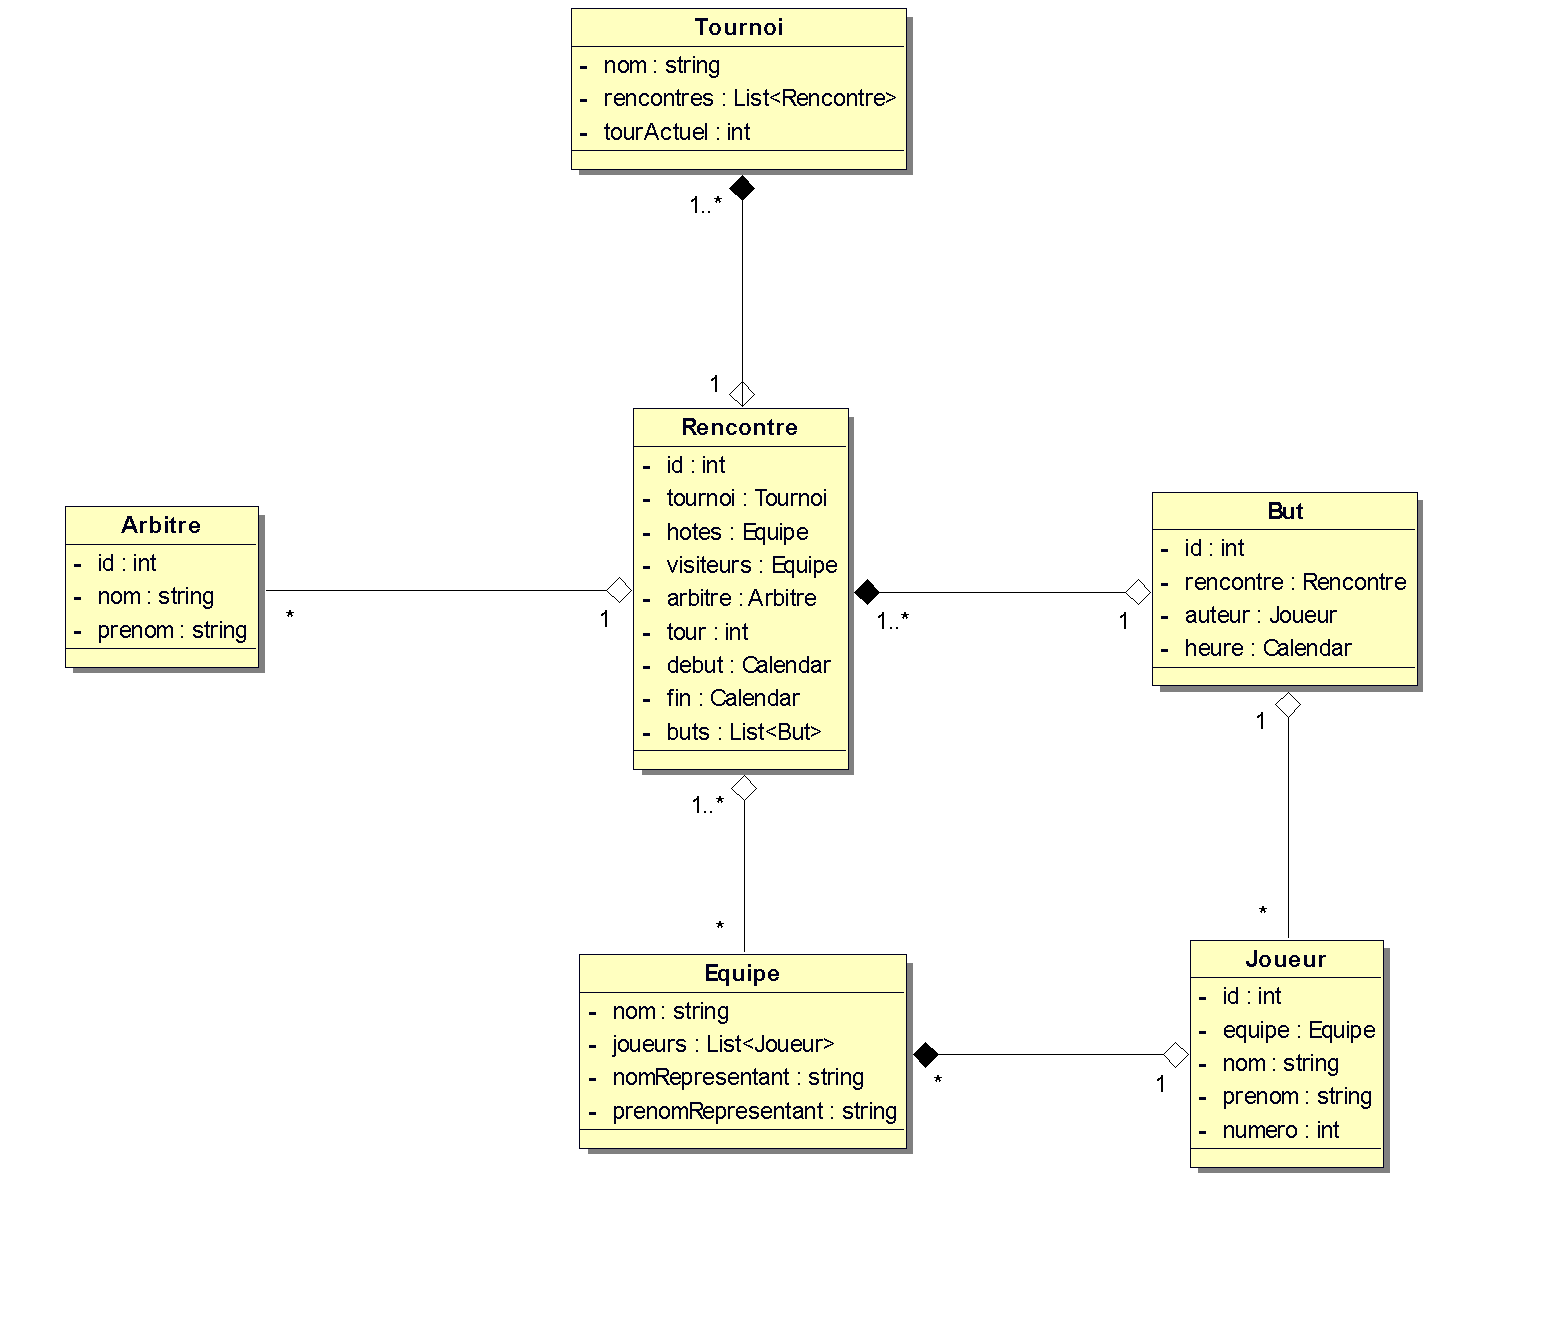
\includegraphics[scale=0.8]{class}}
	      \end{center}
	\legend{\underline{Diagramme de classes du modèle}}
	\end{figure}

Un \textit{Tournoi} est composé d'un nom, d'une liste de rencontres et le tour actuel afin de pouvoir l'incrémenter en temps voulu pour les nouvelles rencontres.

Une \textit{Rencontre} garde une référence vers l'équipe hôte et l'équipe visiteur qui vont s'affronter.
Elle possède aussi l'arbitre, une liste de buts et les dates de début et de fin.
La date de fin est calculée en fonction des buts marqués. On détecte automatiquement s'il y a eu prolongation ou tirs aux buts.

Une \textit{Equipe} contient une liste de joueurs et le nom et prénom du représentant.

Un \textit{But} contient  le joueur qui l'a marqué et la date (heure) associée.
 
Le \textit{Joueur} et l'\textit{Arbitre} sont simplement composés d'un nom et d'un prénom.



\newpage
\subsection{Les EJB}
~\\
Le schéma ci-dessous représente le diagramme de classes de l'EJB Utilisateur créé. \\
	\begin{figure}[hp]
	      \begin{center}
		\fbox{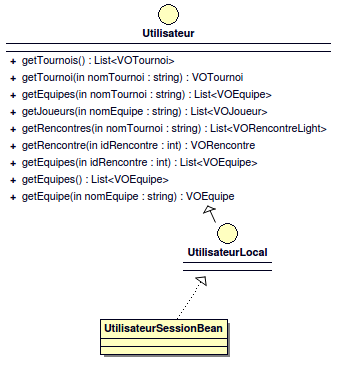
\includegraphics[scale=0.7]{ejb_u}}
	      \end{center}
	\legend{\underline{Diagramme de classes de l'EJB Utilisateur}}	
	\end{figure}
\\

L'EJB Utilisateur se compose de deux interfaces (\textit{Utilisateur} et \textit{UtilisateurLocal}) et d'une classe d'implémentation (\textit{UtilisateurSessionBean}). L'interface \textit{Utilisateur} définit les profils des méthodes implémentées par la classe \textit{UtilisateurSessionBean}. L'interface \textit{UtilisateurLocal} correspond à l'interface locale de l'EJB utilisée par la facade de notre application. L'ensemble des méthodes définies dans cet EJB retournent un Value Object ou une liste de Value Objects. En effet, l'utilisateur ne doit pas être en mesure de connaitre l'ensemble des attributs et méthodes des classes du modèle.

\newpage
Le schéma ci-dessous représente le diagramme de classes de l'EJB Administrateur créé. \\
	\begin{figure}[hp]
	      \begin{center}
		\fbox{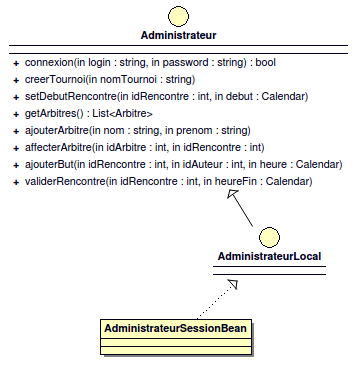
\includegraphics[scale=0.7]{ejb_a}}
	      \end{center}
	\legend{\underline{Diagrammes de classes de l'EJB Administrateur}}	
	\end{figure}
\\

L'EJB Administrateur se compose de deux interfaces (\textit{Administrateur} et \textit{AdministrateurLocal}) et d'une classe d'implémentation (\textit{AdministrateurSessionBean}). L'interface \textit{Administrateur} définit les profils des méthodes implémentées par la classe \textit{AdministrateurSessionBean}. L'interface \textit{AdministrateurLocal} correspond à l'interface locale de l'EJB utilisée par la facade de notre application. Les méthodes définies concernent la connexion de l'administrateur à l'application, la création d'un tournoi ou encore le déroulement des matchs (indication des horaires, affectation des arbitres).

\newpage
Le schéma ci-dessous représente le diagramme de classes de l'EJB Représentant créé. \\
	\begin{figure}[hp]
	      \begin{center}
		\fbox{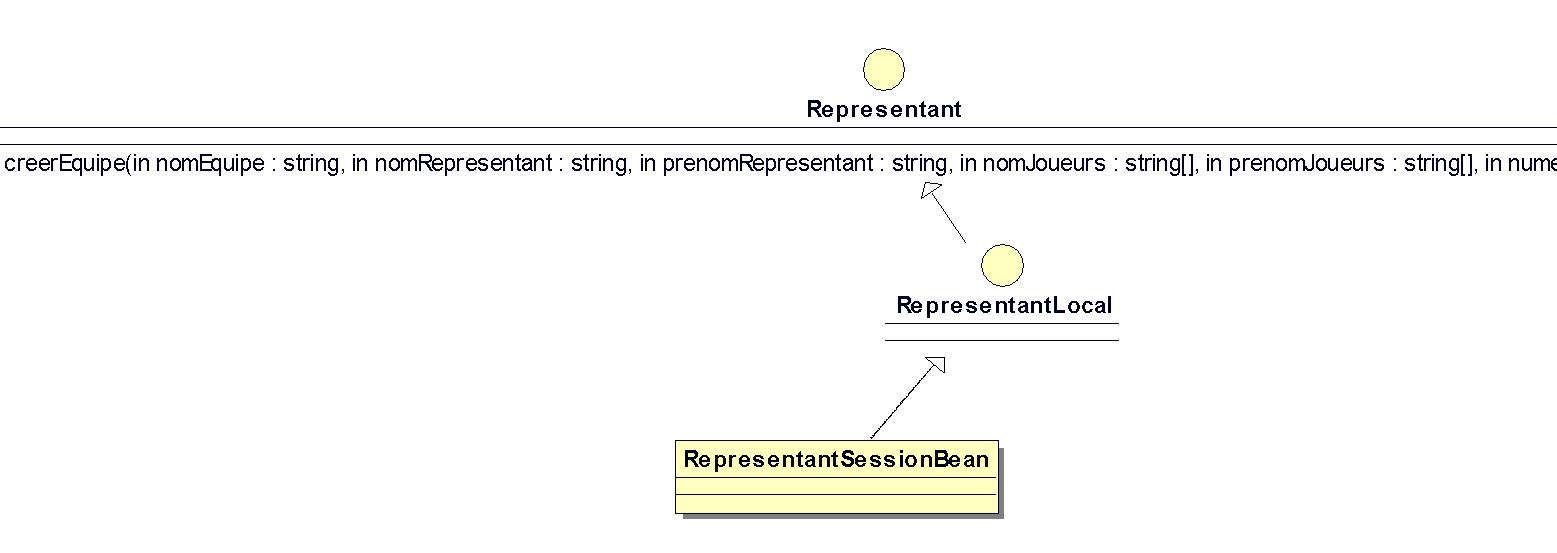
\includegraphics[scale=0.8]{ejb_r}}
	      \end{center}
	\legend{\underline{Diagramme de classes de l'EJB Représentant}}
	\end{figure}
\\
	
L'EJB Représentant se compose de deux interfaces (\textit{Representant} et \textit{RepresentantLocal}) et d'une classe d'implémentation (\textit{RepresentantSessionBean}). L'interface \textit{Representant} définit le profil de la méthode implémentée par la classe \textit{RepresentantSessionBean}. L'interface \textit{RepresentantLocal} correspond à l'interface locale de l'EJB utilisée par la facade de notre application. La méthode définie consiste à la création d'une équipe au sein de l'application.

\newpage
Le schéma ci-dessous représente le diagramme de classes de l'EJB session Facade créé. \\
	\begin{figure}[hp]
	      \begin{center}
		\fbox{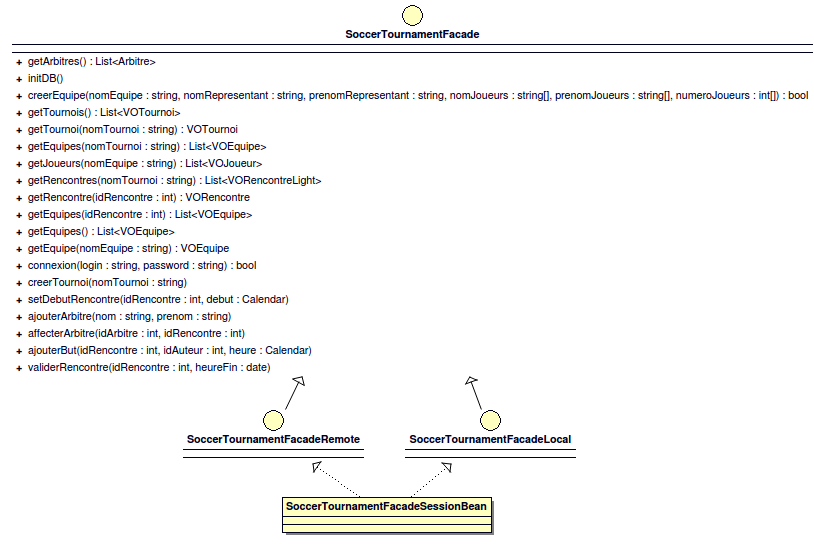
\includegraphics[scale=0.7]{ejb_f}}
	      \end{center}
	\legend{\underline{Diagramme de l'EJB session Facade}}
	\end{figure}	
\\

L'EJB session Facade se compose de trois interfaces (\textit{SoccerTournamentFacade}, \textit{SoccerTournamentFacadeLocal} et \textit{SoccerTournamentFacadeRemote}) et d'une classe d'implémentation (\textit{SoccerTournamentFacadeBean}). L'interface \textit{SoccerTournamentFacadeLocal} correspond à l'interface locale de l'EJB utilisée dans notre application. Nous avons également créé l'interface \textit{SoccerTournamentFacadeRemote} dans le cas où nous devions atteindre la façade à distance. Cet EJB regroupe l'ensemble des méthodes définies dans les EJB créés ainsi qu'une méthode \textit{InitDB()} nous permettant d'initialiser la base de données au lancement de l'application. La base de données se charge ainsi, à l'aide de fichiers XML préalablements remplis. 

\newpage
\subsection{Les Value Objects}
~\\
Le schéma ci-dessous représente le diagramme de classes des Value Objects créés. \\
	\begin{figure}[here]
	      \begin{center}
		\fbox{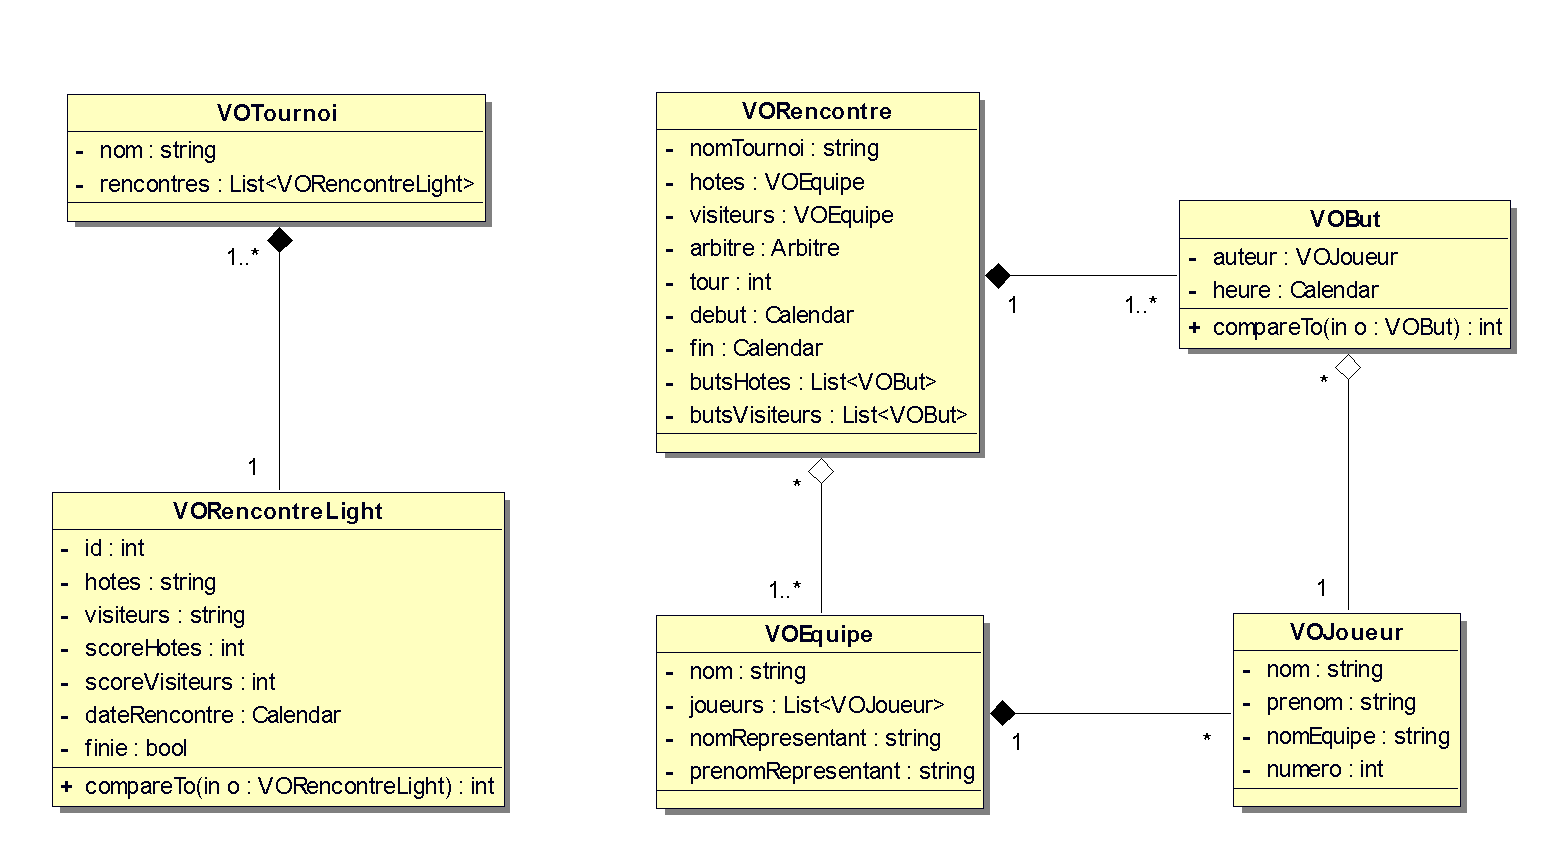
\includegraphics[scale=0.8]{vo}}
	      \end{center}
	\legend{\underline{Diagramme de classes des Value Objects}}
	\end{figure}

Les value objects permettent de ne donner aux jsp que les données nécessaires.
Les notres sont divisés en deux groupes.

La \textbf{VORencontre} possède les informations d'une rencontre et les classes de type \textbf{VOEquipe} et \textbf{VOBut}.
Nous avons gardé la classe \textbf{Arbitre} telle quelle car elle n'avais aucun lien vers les autres classes du modèle et ne représentait donc pas un risque.
La \textbf{VOEquipe} contient une liste de \textbf{VOJoueur} et la \textbf{VOBut} un \textbf{VOJoueur}.
Le \textbf{VOJoueur} est un joueur dans lequel la référence à l'équipe a été remplacée par son nom.

D'un autre coté, nous avons la \textbf{VOTournoi} qui contient une liste de \textbf{VORencontreLight}.
Cette classe, plus légère, ne contient que le nom des équipes et quelques informations telles que les scores et l'état de terminaison de la rencontre.
Il était inutile de garder un lien vers les équipes alors qu'on ne veut afficher que peu d'informations.

\newpage
\section{Diagramme de cas d'utilisation}
~\\
Le schéma ci-dessous représente le diagramme de cas d'utilisation de notre application. \\
	\begin{figure}[hp]
	      \begin{center}
		\fbox{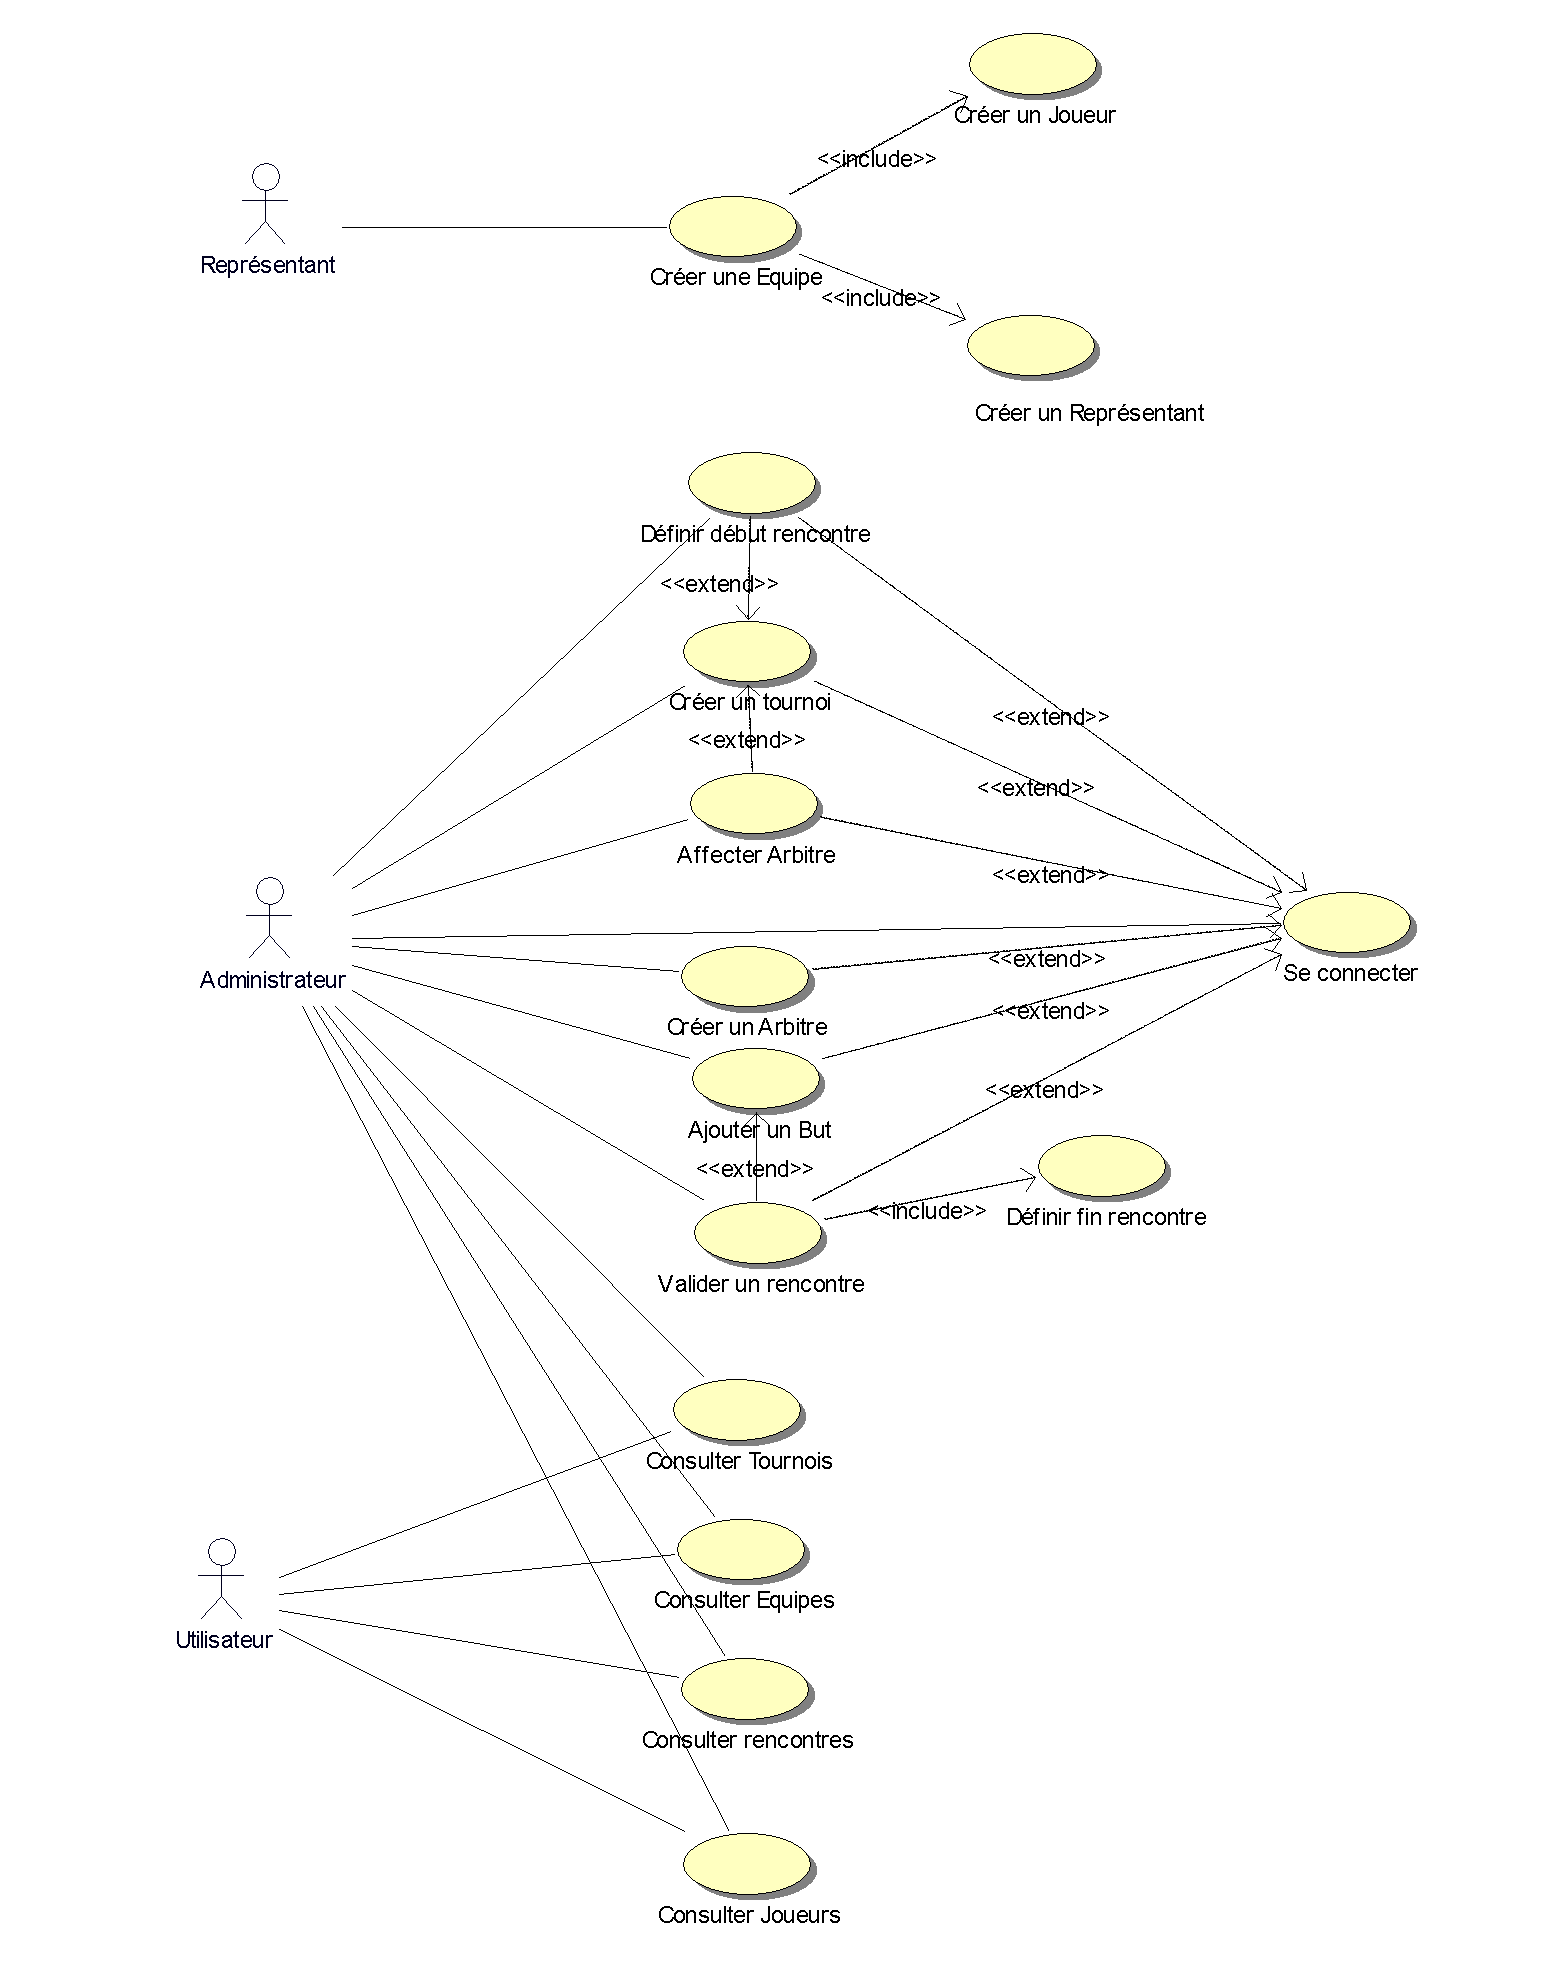
\includegraphics[scale=0.7]{use_cases}}
	      \end{center}
	\legend{\underline{Diagramme de cas d'utilisation}}
	\end{figure}

Ce diagramme nous a permis de définir les différentes EJB et les méthodes nécessaires à chacun.

Pour commencer, le \textbf{Représentant} peut créer une équipe, ce qui crée les joueurs et le représentant.

Ensuite, l'\textbf{Administrateur} peut créer un tournoi, définir le début d'une rencontre y ajouter des buts et la valider.
De plus, il peut créer un arbitre et l'affecter à une rencontre.
Toutes ces actions ne peuvent se faire que s'il s'est connecté auparavant.

Pour finir, l'\textbf{Utilisateur} peut consulter les tournois, les rencontres, les équipes et les joueurs.
L'\textbf{Administrateur} peut aussi effectuer les actions de l'\textbf{Utilisateur}.

\newpage
\section{Schéma synthétique de l'application}
~\\
Le schéma ci-dessous représente le schéma synthétique de l'application développée. \\
	\begin{figure}[hp]
	      \begin{center}
		\fbox{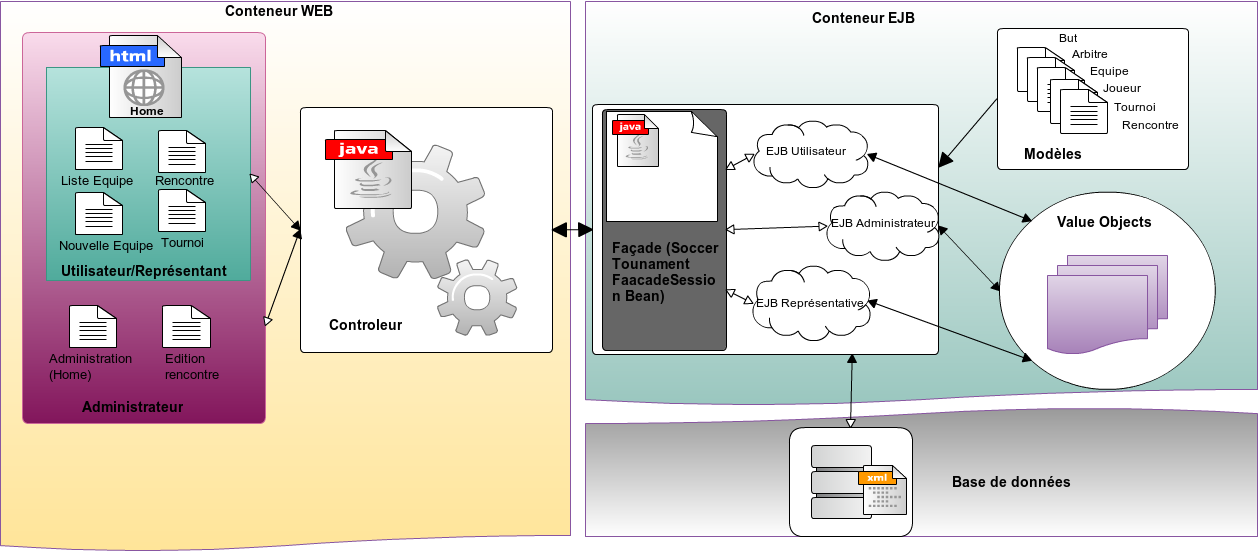
\includegraphics[width=18cm]{AAR}}
	      \end{center}
	\legend{\underline{Schéma synthétique de l'application}}
	\end{figure}

\newpage
\chapter{Répartition du travail}
\section{Gestion du temps de travail}
~\\
Le diagramme de Gantt ci-dessous présente la répartition du travail tout au long du projet. \\
	\begin{figure}[hp]
	      \begin{center}
		\fbox{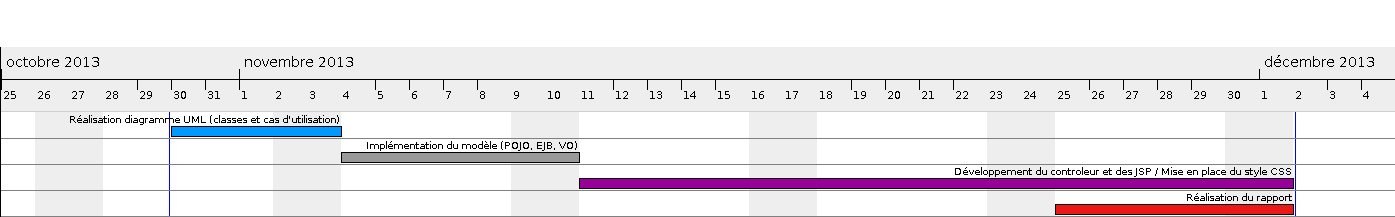
\includegraphics[width=18cm]{gantt}}
	      \end{center}
	\legend{\underline{Gestion du temps de travail}}
	\end{figure}
\\

La première semaine de travail fut consacrée à l'analyse UML et à l'élaboration des diagrammes de classes et des diagrammes de cas d'utilisation. Une fois cela fait, nous avons débuté l'implémentation du modèle de l'application à savoir les objets POJO, les EJB ainsi que les Value Objects. Le développpement du controleur et des vues utilisateurs et administrateurs a été réalisé ensuite jusqu'à la fin du projet. Le rapport, quant à lui, a été rédigé dans la dernière semaine de travail.\\

\section{Répartition des tâches}
~\\

L'ensemble du groupe a travaillé sur la réalisation de l'analyse UML et la détermination des différentes classes utiles dans l'application.
Geoffrey s'est vu attribuer l'EJB Utilisateur alors que Zo s'est vu faire le Représentant et une partie de l'Administrateur.
Zo et Willy se sont occupés des entités.
Geoffrey et Willy se sont chargés de l'implémentation des Value Objects.
Willy a également créé le jeu de test au travers de fichiers XML permettant de charger la base de données et la validation de rencontre.

Au niveau de la partie web, Zo s'est principalement occupé de la mise en place du CSS et du développement des JSP  \textit{newteam}, \textit{index}, \textit{login} et \textit{team} pour la visualisation des équipes, des joueurs, la création d'une équipe et la connexion.
Willy a travaillé sur \textit{adminmatch}, qui permet à l'administrateur d'éditer une rencontre, une taglib permettant d'afficher le diagramme d'un tournoi et la réalisation d'une foire aux questions.
Geoffrey a développé la JSP \textit{match} coté utilisateur, affichant l'ensemble des informations relatifs à une rencontre.

L'ensemble du groupe a contribué à la création du controleur ainsi que tu déboguage des différentes classes et jsp et la rédaction du rapport.
  
\chapter{Guide d'utilisation}


L'application est accessible par l'URL suivante :
\begin{center}
\textit{http://localhost:8080/SoccerTournamentWeb/}
\end{center}

Vous devez au préalable lancer l'application sur un serveur d'application JBoss.
Selon votre configuration, le port de l'application peut varier.
\\

Pour accéder à notre foire aux questions (qui fait office de manuel), il vous suffit de cliquer sur l'icône en forme de point d'interrogation.
Des renseignements sont aussi disponibles pour l'administrateur sur cette même page, il faut pour cela vous connecter.
Pour vous connecter en tant qu'administrateur, il vous suffit de cliquer sur l'icône en forme de clé et d'entrer les renseignements suivants :
\begin{center}
\textbf{Login} : admin
\\
\textbf{Password} : root 
\end{center}

\chapter*{Conclusion}

Ce projet aura permis de mettre en oeuvre les connaissances vues tout au long du semestre. Le groupe a pu améliorer ses compétences dans l'utilisation de la technologie J2EE et a acquis les principales notions de persistence d'objets, dans une base de données, avec l'usage des EJB. L'intérêt des Value Objects a été compris lors de ce projet et, les membres du groupe ont également renforcés leurs compétences dans le domaine du Web en travaillant sur un controleur et ses JSP. 

\end{document}
